\documentclass[main.tex]{subfiles}
\begin{document}
\begin{figure}[ht]
    \centering
    \begin{subfigure}{0.3\textwidth}
        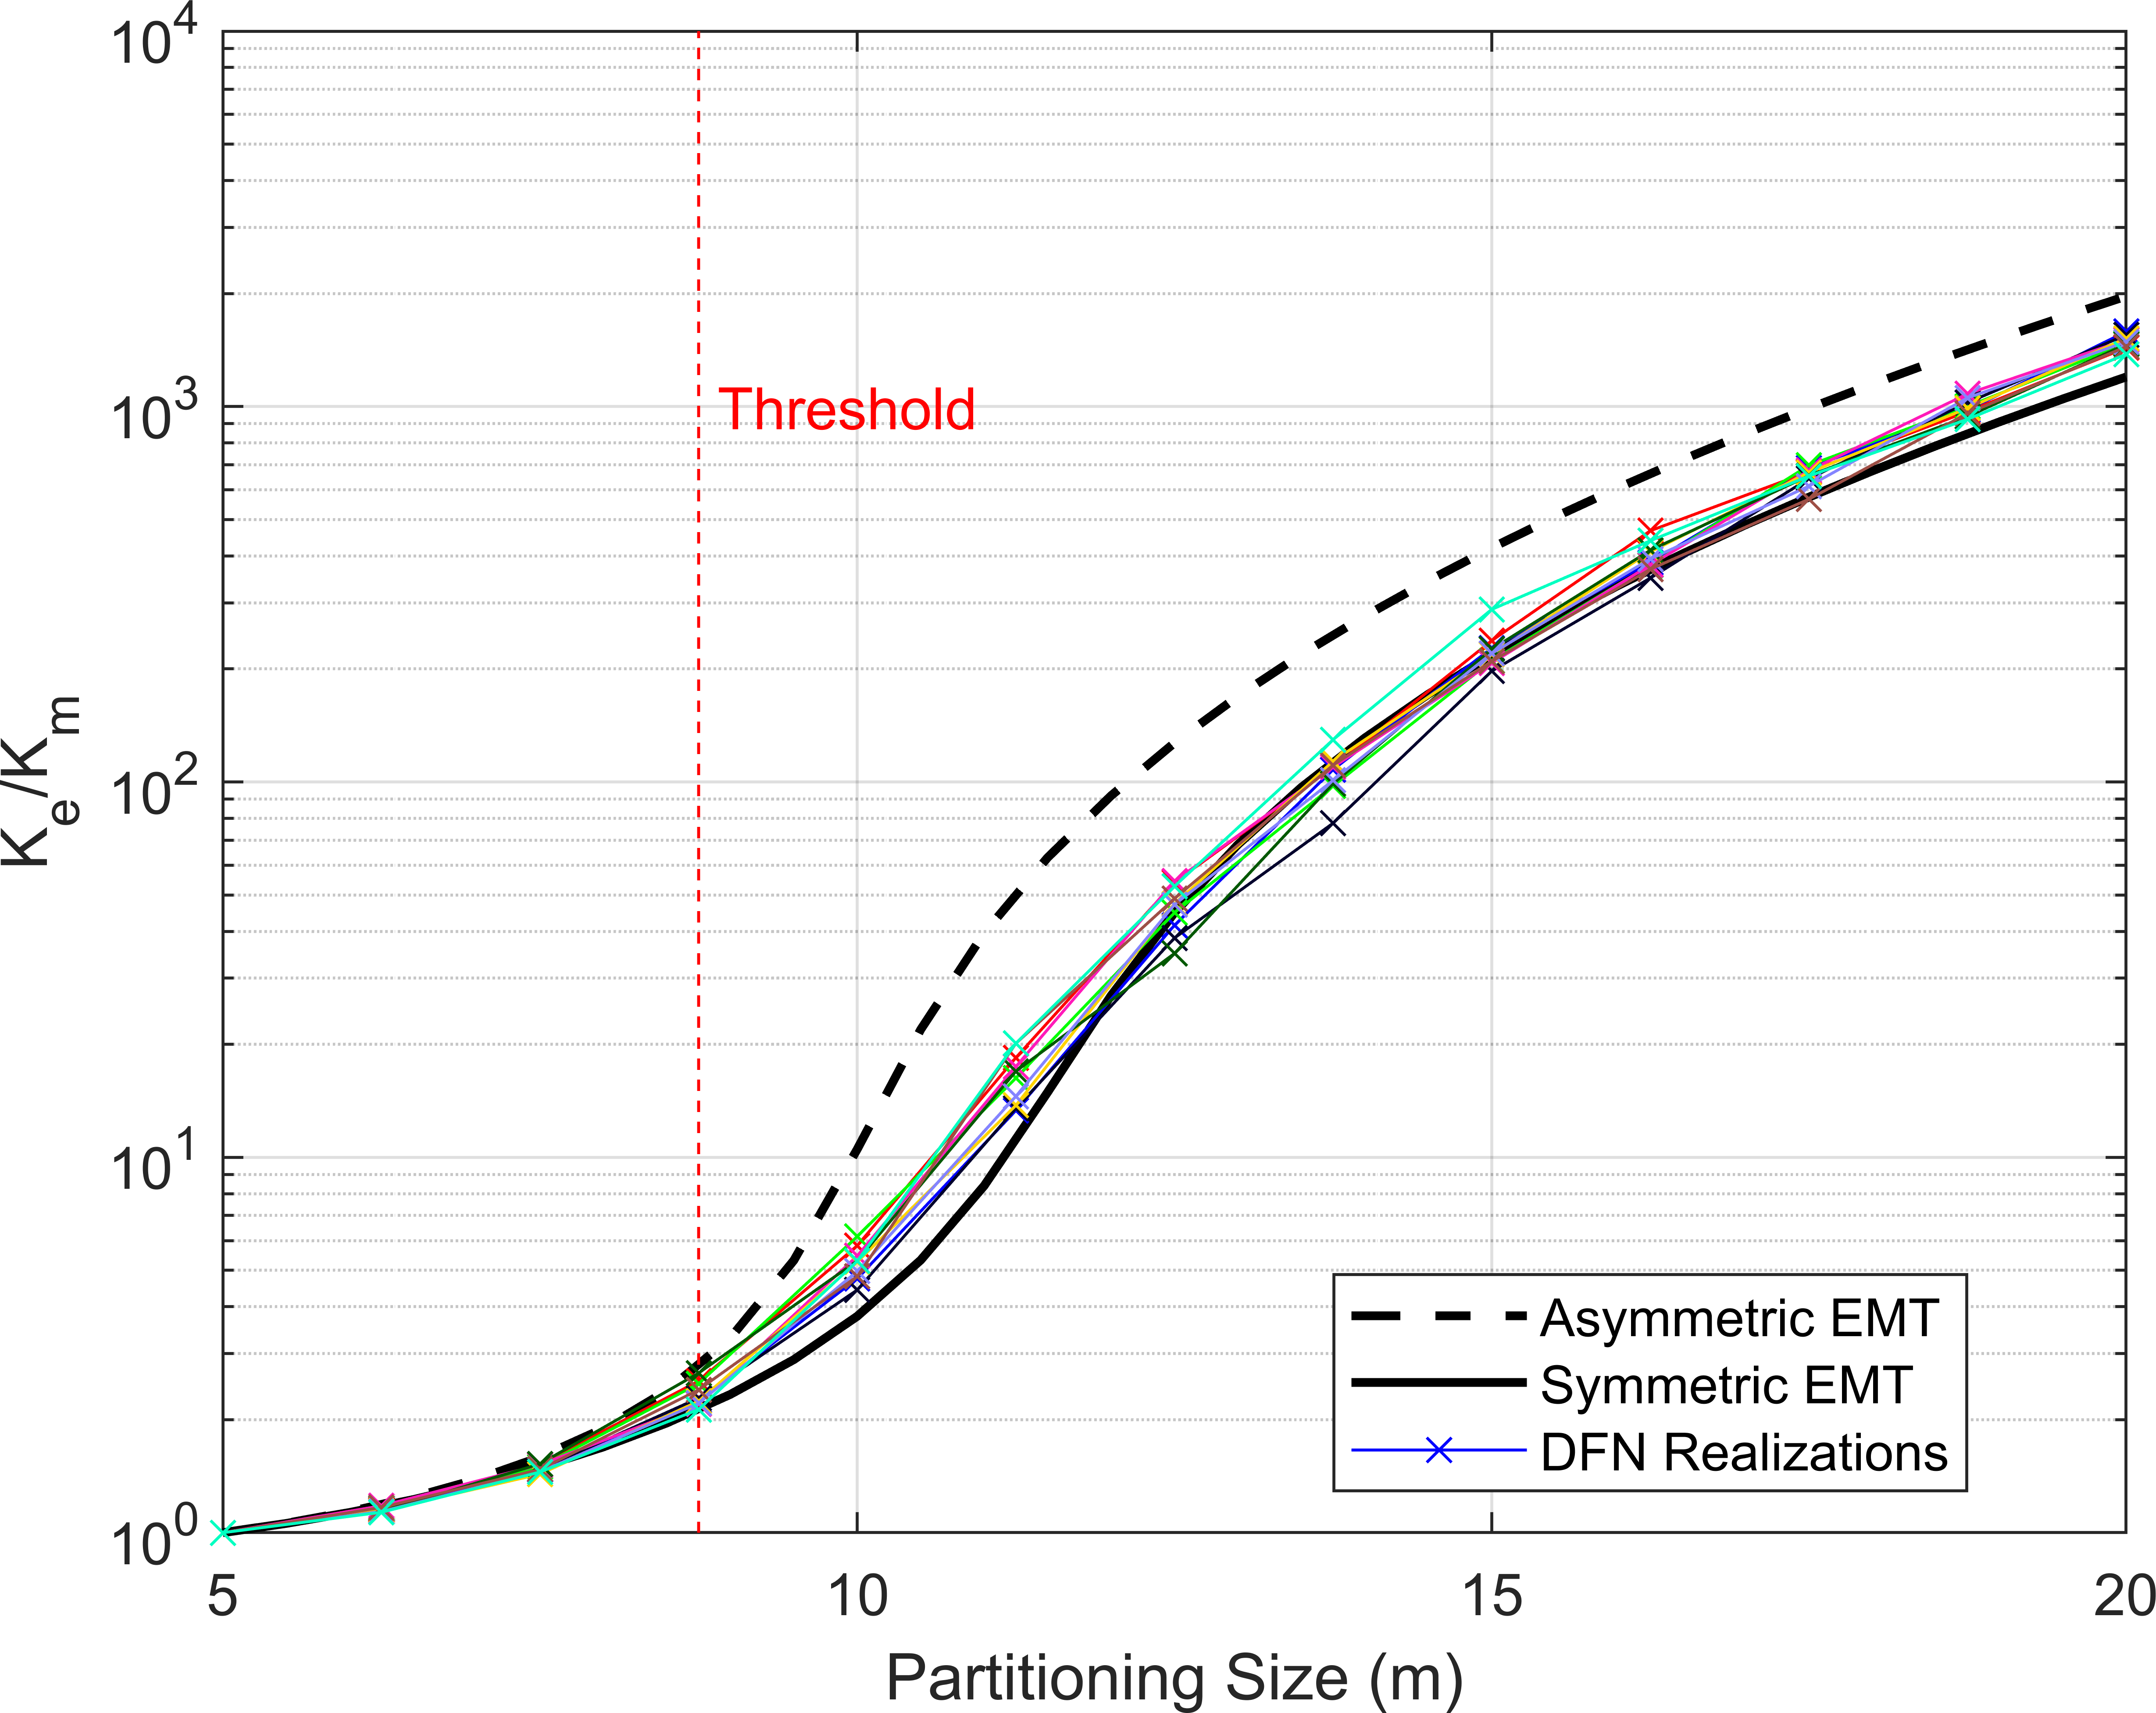
\includegraphics[width=\textwidth]{FSU/Plot_FSU_Case_01_nohead.png}
        \subcaption{Case A: Base parameters}
        \label{fig:FSU_A}
    \end{subfigure}
    \begin{subfigure}{0.3\textwidth}
        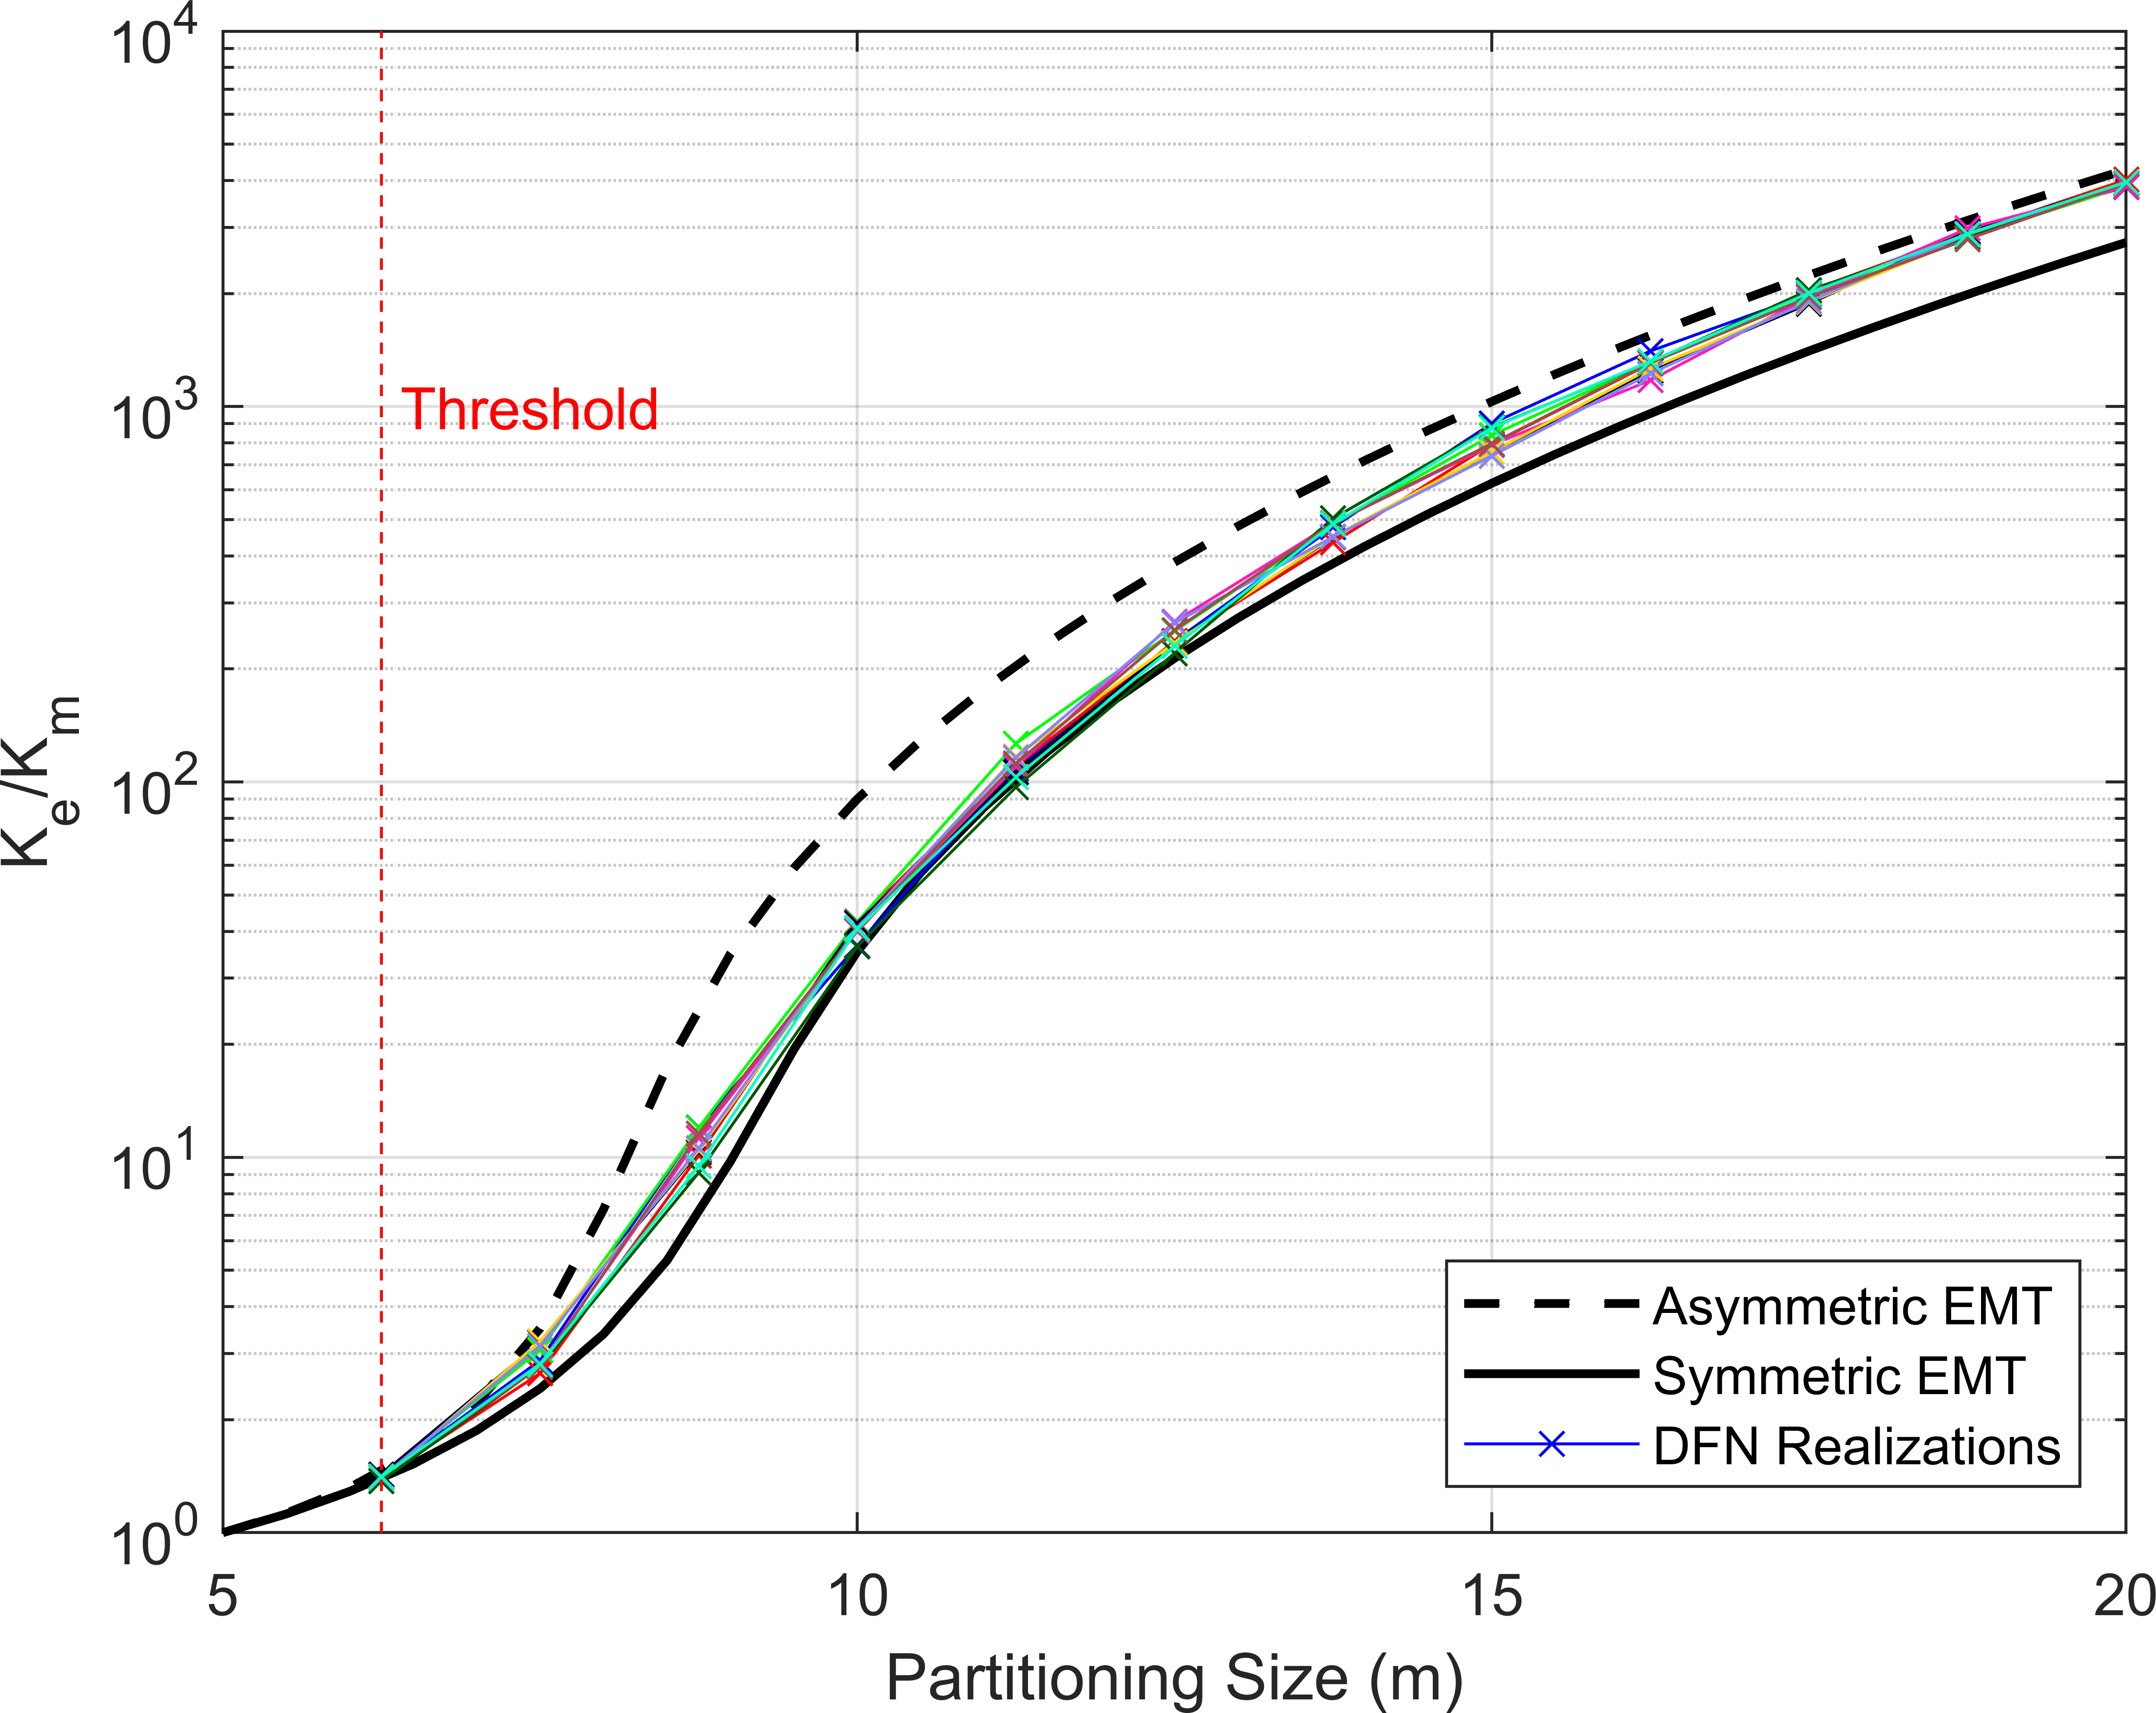
\includegraphics[width=\textwidth]{FSU/Plot_FSU_Case_03_nohead.png}
        \subcaption{Case B: 2x Density}
        \label{fig:FSU_B}
    \end{subfigure}
    \begin{subfigure}{0.3\textwidth}
        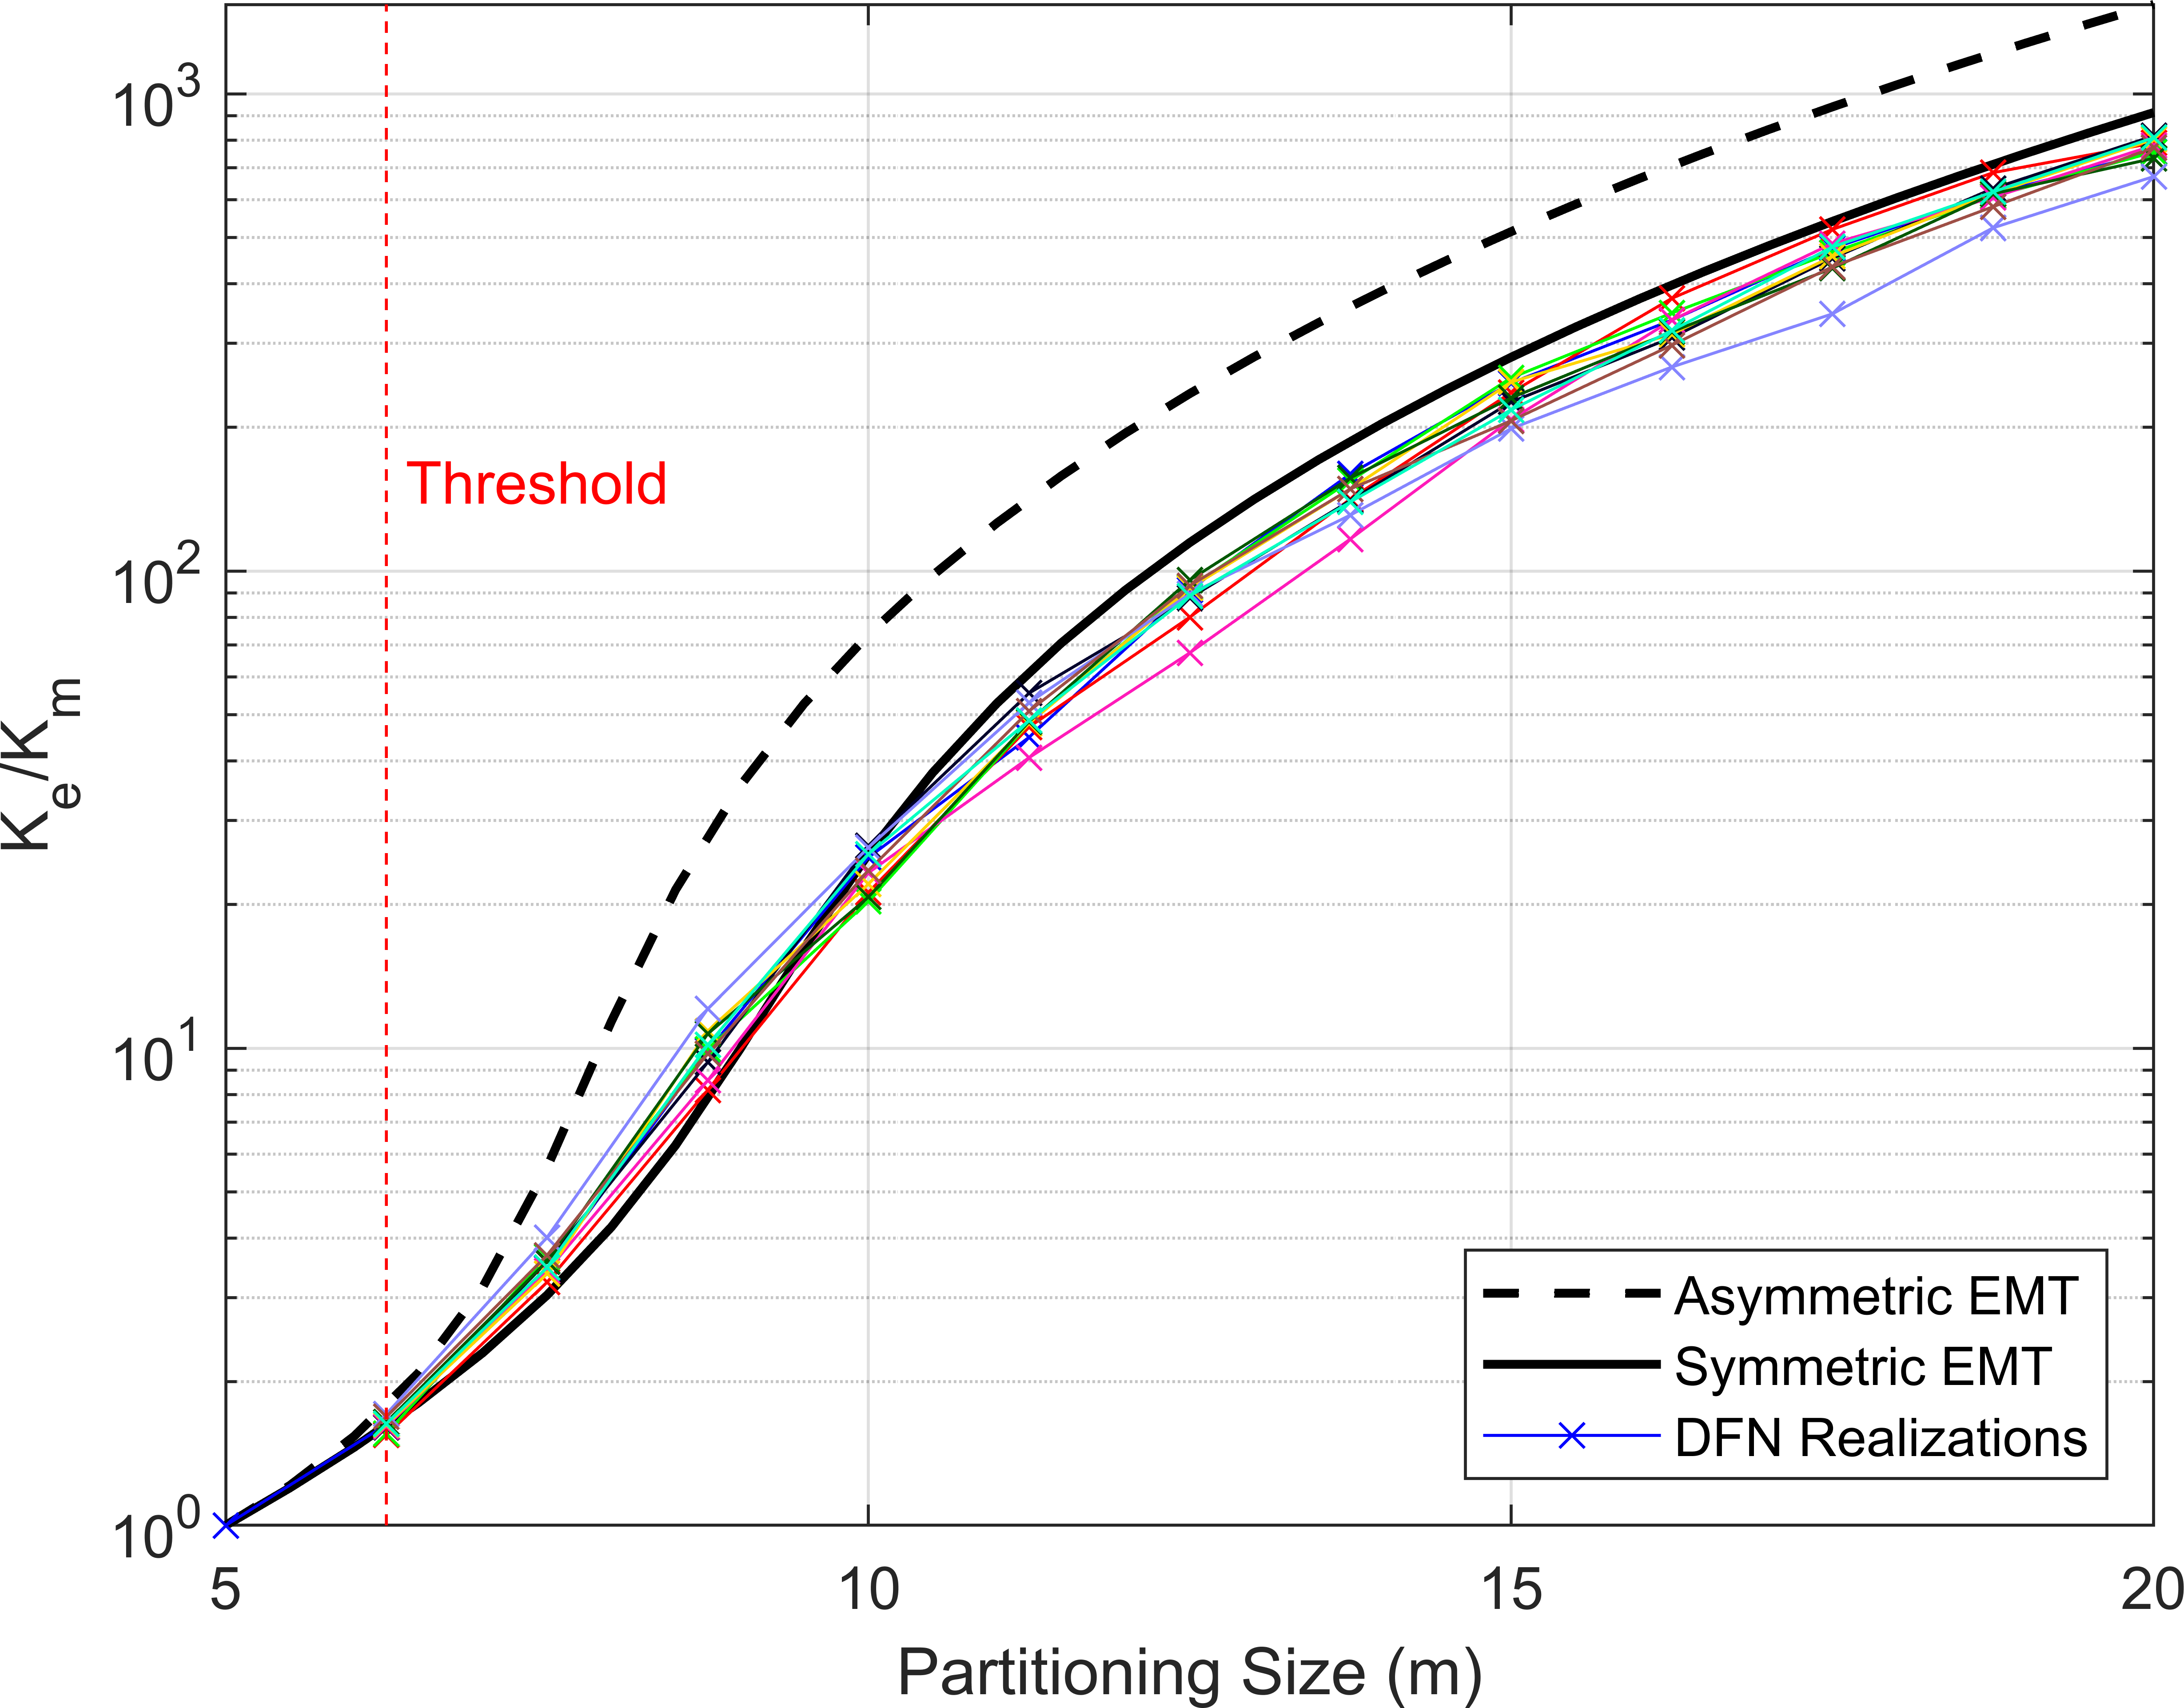
\includegraphics[width=\textwidth]{FSU/Plot_FSU_Case_05_nohead.png}
        \subcaption{Case C: 2x Size Exponent}
        \label{fig:FSU_C}
    \end{subfigure}
    \begin{subfigure}{0.3\textwidth}
        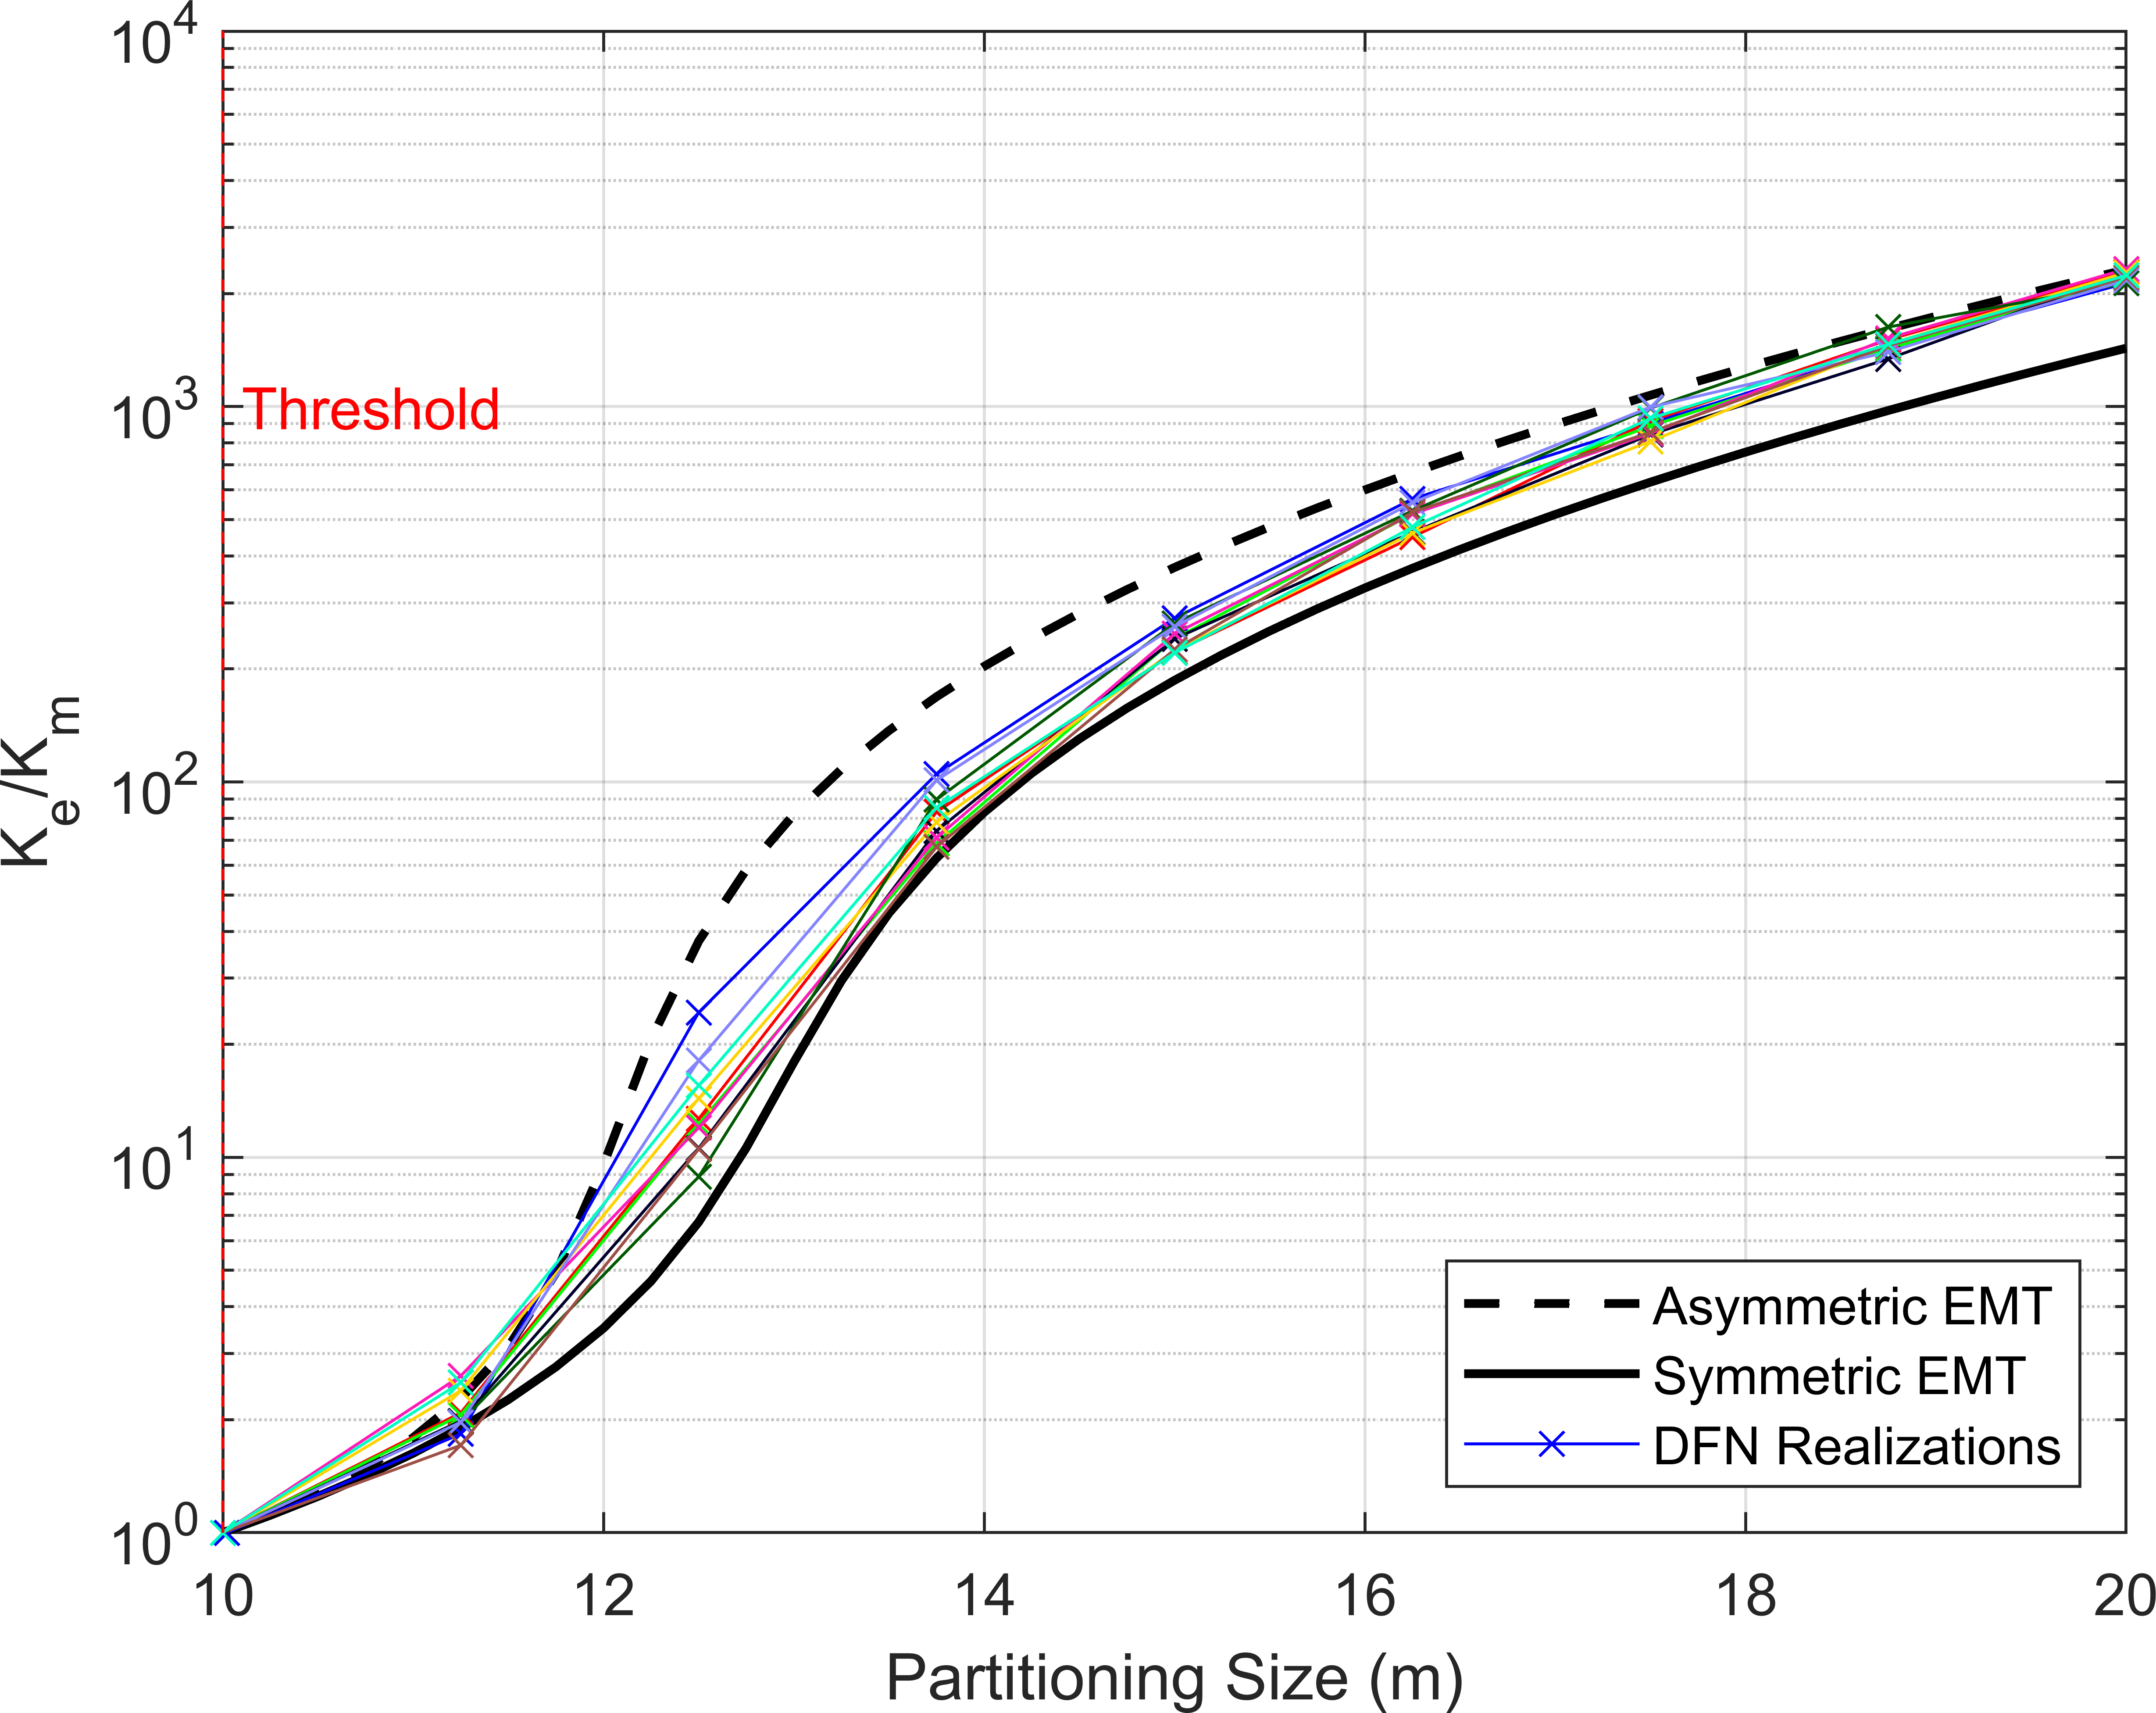
\includegraphics[width=\textwidth]{FSU/Plot_FSU_Case_07_nohead.png}
        \subcaption{Case D: 2x Min Size}
        \label{fig:FSU_D}
    \end{subfigure}
    \begin{subfigure}{0.3\textwidth}
        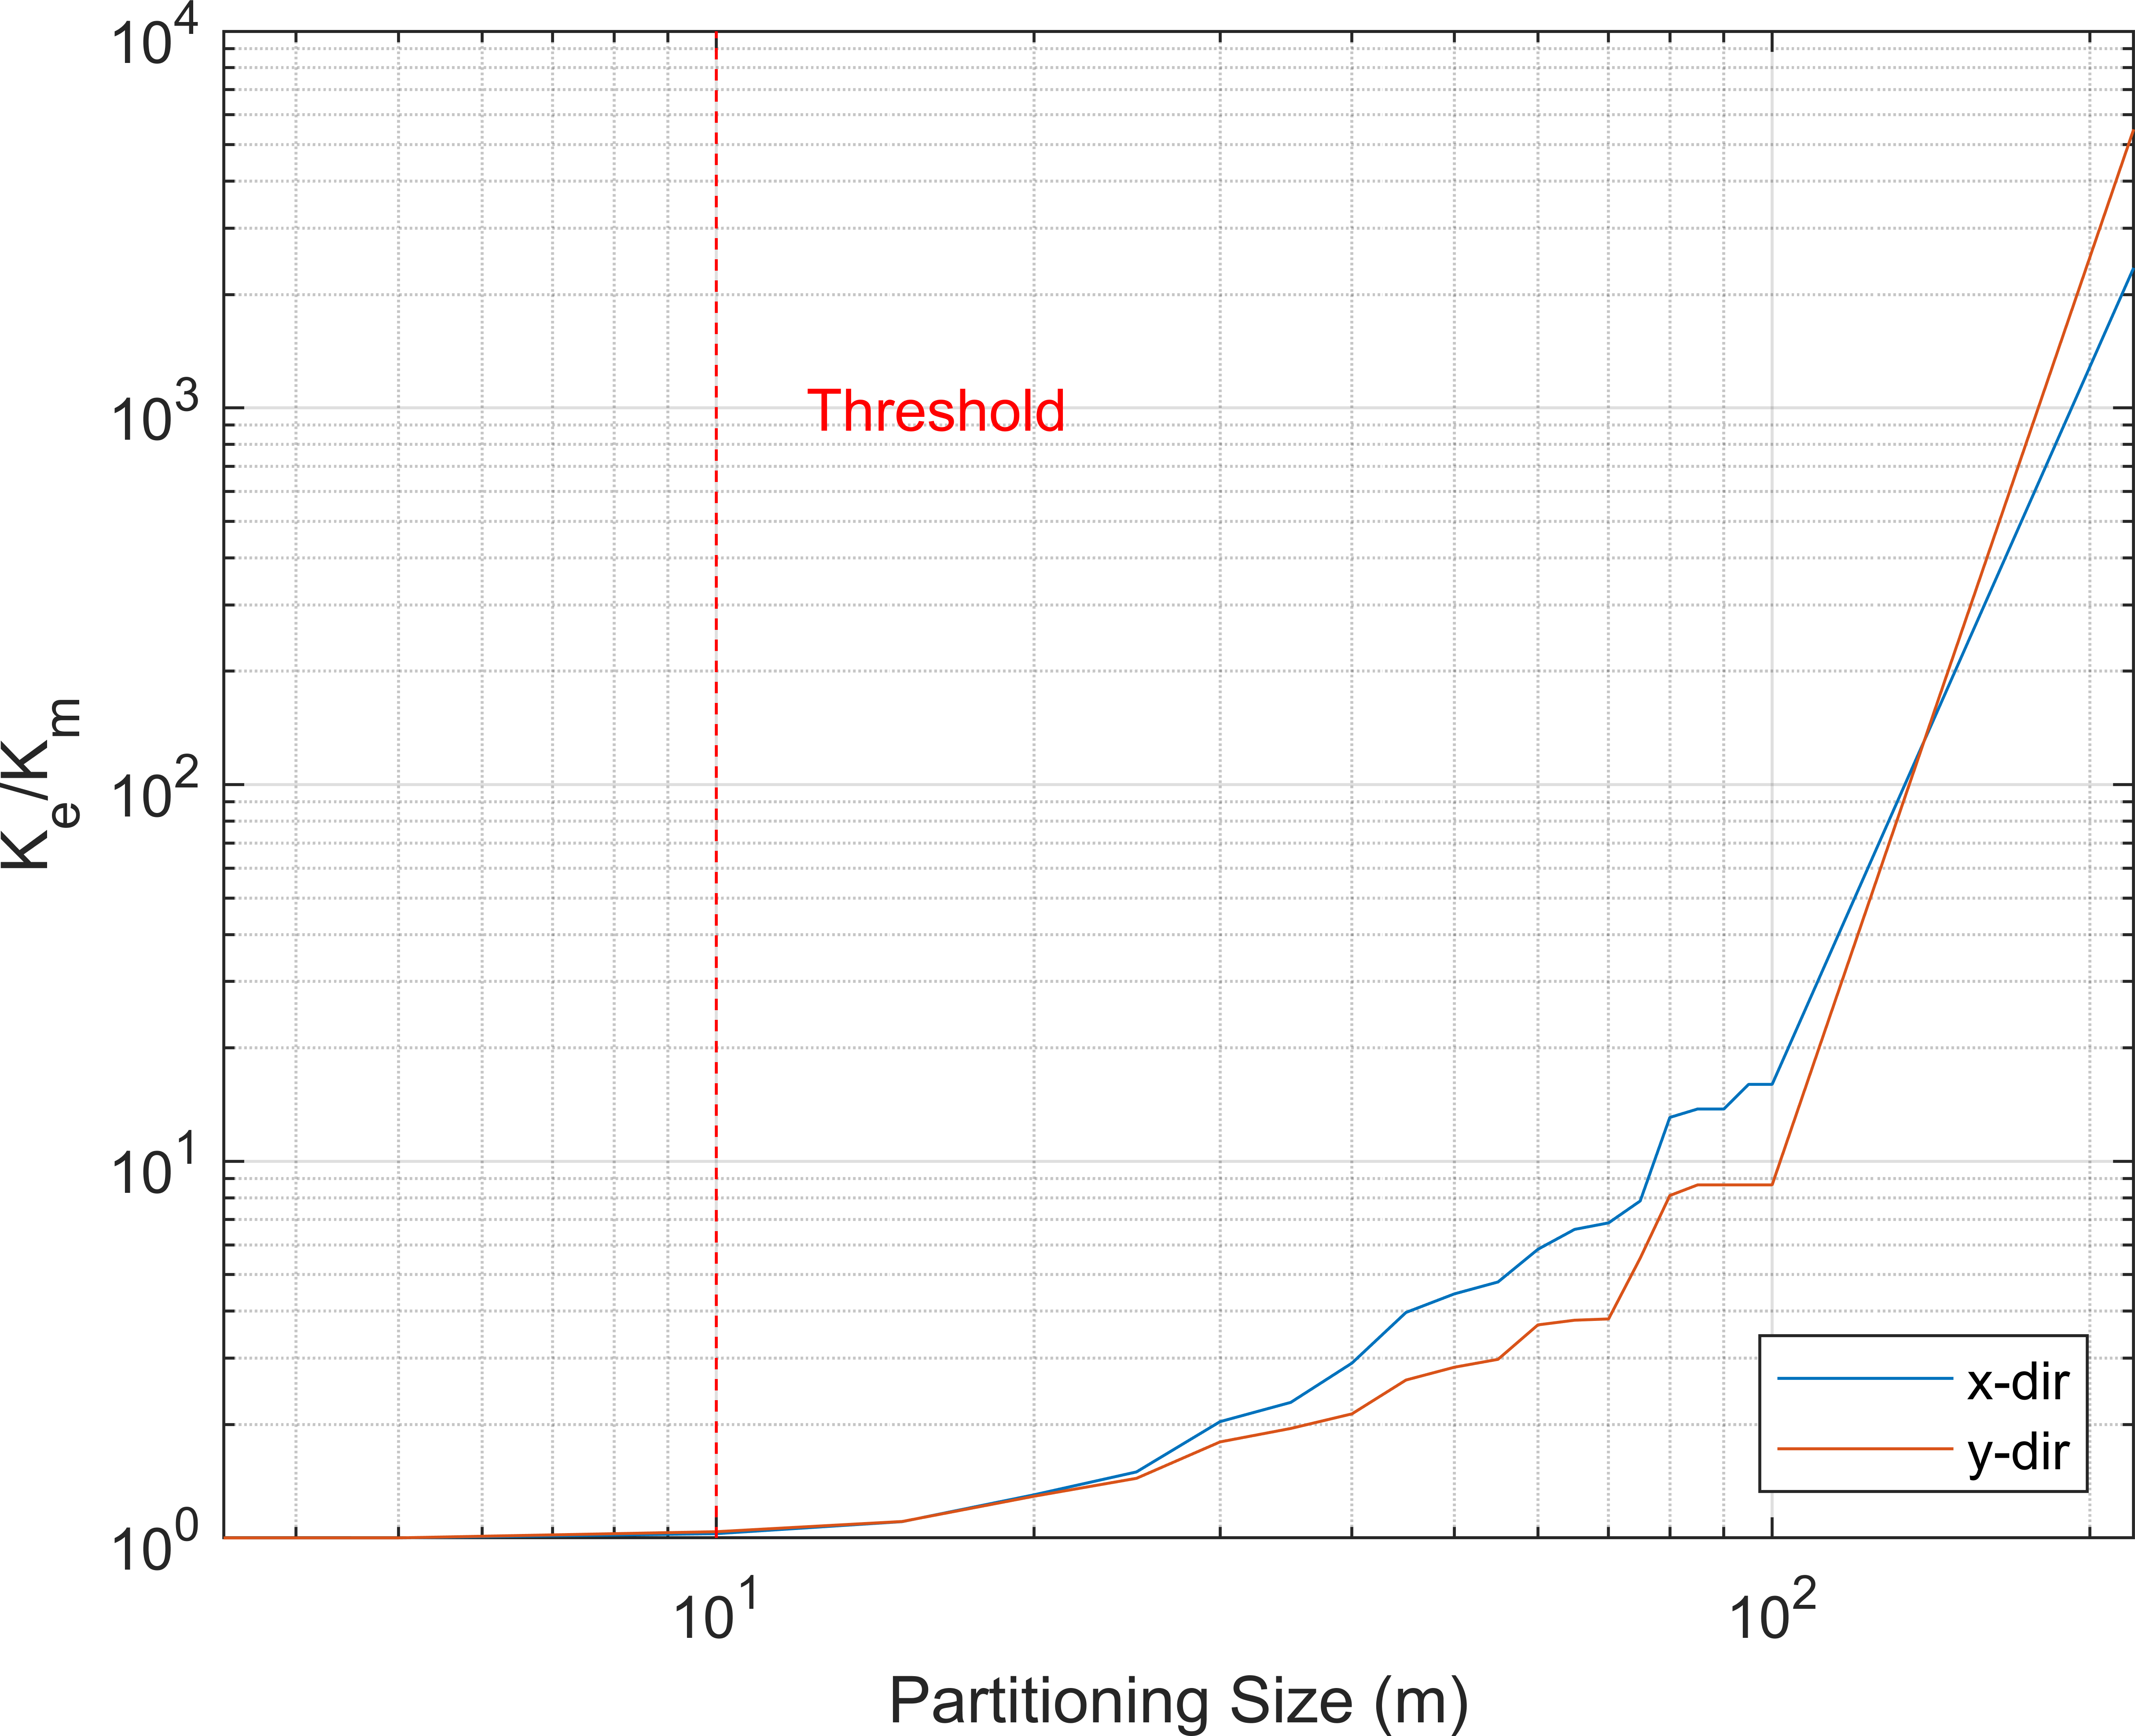
\includegraphics[width=\textwidth]{FSU/Apodi2_FSU_nohead.png}
        \subcaption{Apodi 2}
        \label{fig:FSU_A2}
    \end{subfigure}
    \begin{subfigure}{0.3\textwidth}
        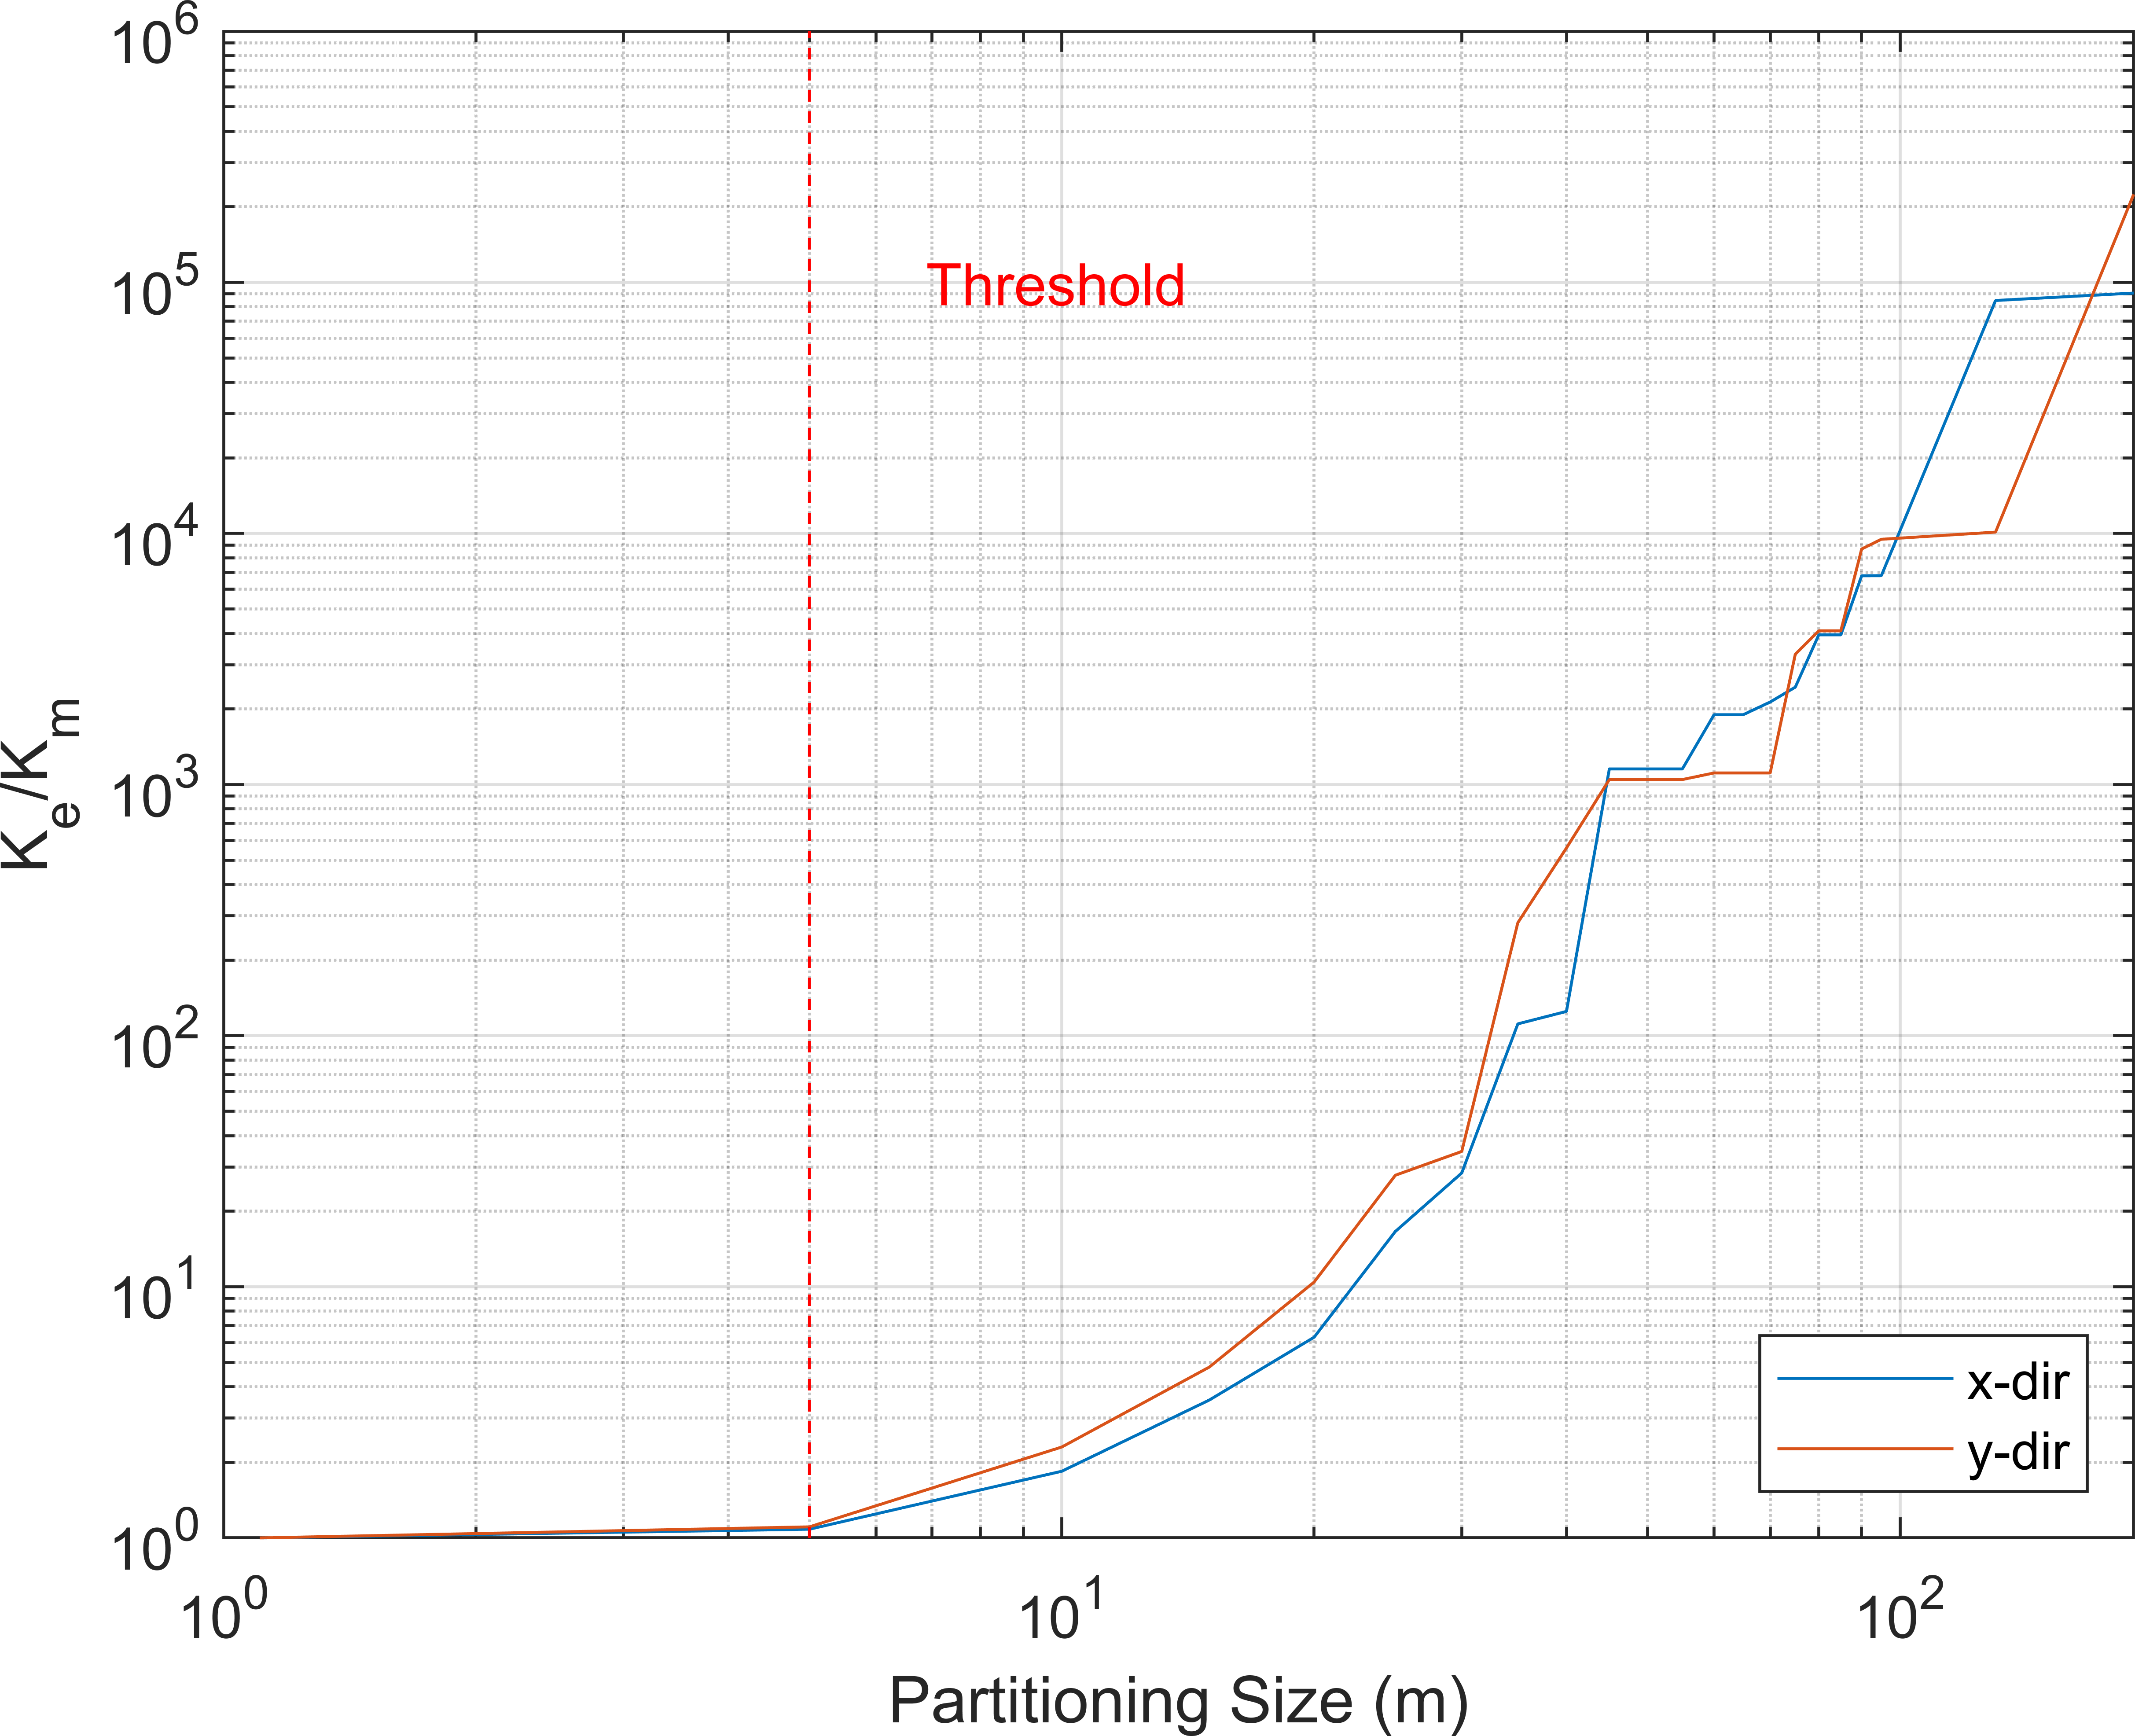
\includegraphics[width=\textwidth]{FSU/Apodi4_FSU_nohead.png}
        \subcaption{Apodi 4}
        \label{fig:FSU_A4}
    \end{subfigure}
    \caption{Fracture Subset Upscaling. (a)-(d) correspond to generated 3D DFNs. To capture variations due to the power law size distribution used, 10 stochastic realizations were created for each case. (e)-(f) correspond to outcrop fracture data. Threshold partitioning sizes are identified from Figure \ref{fig:DD}.}
    \label{fig:FSU}
\end{figure}
\end{document}